\documentclass{ximera}  


%\usepackage{todonotes}
%\usepackage{mathtools} %% Required for wide table Curl and Greens
%\usepackage{cuted} %% Required for wide table Curl and Greens
\newcommand{\todo}{}

\usepackage{esint} % for \oiint
\ifxake%%https://math.meta.stackexchange.com/questions/9973/how-do-you-render-a-closed-surface-double-integral
\renewcommand{\oiint}{{\large\bigcirc}\kern-1.56em\iint}
\fi


\graphicspath{
  {./}
  {jpg}
  {ximeraTutorial/}
  {basicPhilosophy/}
  {functionsOfSeveralVariables/}
  {normalVectors/}
  {lagrangeMultipliers/}
  {vectorFields/}
  {greensTheorem/}
  {shapeOfThingsToCome/}
  {dotProducts/}
  {partialDerivativesAndTheGradientVector/}
  {../productAndQuotientRules/exercises/}
  {../motionAndPathsInSpace/exercises/}
  {../normalVectors/exercisesParametricPlots/}
  {../continuityOfFunctionsOfSeveralVariables/exercises/}
  {../partialDerivativesAndTheGradientVector/exercises/}
  {../directionalDerivativeAndChainRule/exercises/}
  {../commonCoordinates/exercisesCylindricalCoordinates/}
  {../commonCoordinates/exercisesSphericalCoordinates/}
  {../greensTheorem/exercisesCurlAndLineIntegrals/}
  {../greensTheorem/exercisesDivergenceAndLineIntegrals/}
  {../shapeOfThingsToCome/exercisesDivergenceTheorem/}
  {../greensTheorem/}
  {../shapeOfThingsToCome/}
  {../separableDifferentialEquations/exercises/}
  {vectorFields/}
}

\newcommand{\mooculus}{\textsf{\textbf{MOOC}\textnormal{\textsf{ULUS}}}}

\usepackage{tkz-euclide}\usepackage{tikz}
\usepackage{tikz-cd}
\usetikzlibrary{arrows}
\tikzset{>=stealth,commutative diagrams/.cd,
  arrow style=tikz,diagrams={>=stealth}} %% cool arrow head
\tikzset{shorten <>/.style={ shorten >=#1, shorten <=#1 } } %% allows shorter vectors

\usetikzlibrary{backgrounds} %% for boxes around graphs
\usetikzlibrary{shapes,positioning}  %% Clouds and stars
\usetikzlibrary{matrix} %% for matrix
\usepgfplotslibrary{polar} %% for polar plots
\usepgfplotslibrary{fillbetween} %% to shade area between curves in TikZ
\usetkzobj{all}
\usepackage[makeroom]{cancel} %% for strike outs
%\usepackage{mathtools} %% for pretty underbrace % Breaks Ximera
%\usepackage{multicol}
\usepackage{pgffor} %% required for integral for loops



%% http://tex.stackexchange.com/questions/66490/drawing-a-tikz-arc-specifying-the-center
%% Draws beach ball
\tikzset{pics/carc/.style args={#1:#2:#3}{code={\draw[pic actions] (#1:#3) arc(#1:#2:#3);}}}



\usepackage{array}
\setlength{\extrarowheight}{+.1cm}
\newdimen\digitwidth
\settowidth\digitwidth{9}
\def\divrule#1#2{
\noalign{\moveright#1\digitwidth
\vbox{\hrule width#2\digitwidth}}}





\newcommand{\RR}{\mathbb R}
\newcommand{\R}{\mathbb R}
\newcommand{\N}{\mathbb N}
\newcommand{\Z}{\mathbb Z}

\newcommand{\sagemath}{\textsf{SageMath}}


%\renewcommand{\d}{\,d\!}
\renewcommand{\d}{\mathop{}\!d}
\newcommand{\dd}[2][]{\frac{\d #1}{\d #2}}
\newcommand{\pp}[2][]{\frac{\partial #1}{\partial #2}}
\renewcommand{\l}{\ell}
\newcommand{\ddx}{\frac{d}{\d x}}

\newcommand{\zeroOverZero}{\ensuremath{\boldsymbol{\tfrac{0}{0}}}}
\newcommand{\inftyOverInfty}{\ensuremath{\boldsymbol{\tfrac{\infty}{\infty}}}}
\newcommand{\zeroOverInfty}{\ensuremath{\boldsymbol{\tfrac{0}{\infty}}}}
\newcommand{\zeroTimesInfty}{\ensuremath{\small\boldsymbol{0\cdot \infty}}}
\newcommand{\inftyMinusInfty}{\ensuremath{\small\boldsymbol{\infty - \infty}}}
\newcommand{\oneToInfty}{\ensuremath{\boldsymbol{1^\infty}}}
\newcommand{\zeroToZero}{\ensuremath{\boldsymbol{0^0}}}
\newcommand{\inftyToZero}{\ensuremath{\boldsymbol{\infty^0}}}



\newcommand{\numOverZero}{\ensuremath{\boldsymbol{\tfrac{\#}{0}}}}
\newcommand{\dfn}{\textbf}
%\newcommand{\unit}{\,\mathrm}
\newcommand{\unit}{\mathop{}\!\mathrm}
\newcommand{\eval}[1]{\bigg[ #1 \bigg]}
\newcommand{\seq}[1]{\left( #1 \right)}
\renewcommand{\epsilon}{\varepsilon}
\renewcommand{\phi}{\varphi}


\renewcommand{\iff}{\Leftrightarrow}

\DeclareMathOperator{\arccot}{arccot}
\DeclareMathOperator{\arcsec}{arcsec}
\DeclareMathOperator{\arccsc}{arccsc}
\DeclareMathOperator{\si}{Si}
\DeclareMathOperator{\scal}{scal}
\DeclareMathOperator{\sign}{sign}


%% \newcommand{\tightoverset}[2]{% for arrow vec
%%   \mathop{#2}\limits^{\vbox to -.5ex{\kern-0.75ex\hbox{$#1$}\vss}}}
\newcommand{\arrowvec}[1]{{\overset{\rightharpoonup}{#1}}}
%\renewcommand{\vec}[1]{\arrowvec{\mathbf{#1}}}
\renewcommand{\vec}[1]{{\overset{\boldsymbol{\rightharpoonup}}{\mathbf{#1}}}\hspace{0in}}

\newcommand{\point}[1]{\left(#1\right)} %this allows \vector{ to be changed to \vector{ with a quick find and replace
\newcommand{\pt}[1]{\mathbf{#1}} %this allows \vec{ to be changed to \vec{ with a quick find and replace
\newcommand{\Lim}[2]{\lim_{\point{#1} \to \point{#2}}} %Bart, I changed this to point since I want to use it.  It runs through both of the exercise and exerciseE files in limits section, which is why it was in each document to start with.

\DeclareMathOperator{\proj}{\mathbf{proj}}
\newcommand{\veci}{{\boldsymbol{\hat{\imath}}}}
\newcommand{\vecj}{{\boldsymbol{\hat{\jmath}}}}
\newcommand{\veck}{{\boldsymbol{\hat{k}}}}
\newcommand{\vecl}{\vec{\boldsymbol{\l}}}
\newcommand{\uvec}[1]{\mathbf{\hat{#1}}}
\newcommand{\utan}{\mathbf{\hat{t}}}
\newcommand{\unormal}{\mathbf{\hat{n}}}
\newcommand{\ubinormal}{\mathbf{\hat{b}}}

\newcommand{\dotp}{\bullet}
\newcommand{\cross}{\boldsymbol\times}
\newcommand{\grad}{\boldsymbol\nabla}
\newcommand{\divergence}{\grad\dotp}
\newcommand{\curl}{\grad\cross}
%\DeclareMathOperator{\divergence}{divergence}
%\DeclareMathOperator{\curl}[1]{\grad\cross #1}
\newcommand{\lto}{\mathop{\longrightarrow\,}\limits}

\renewcommand{\bar}{\overline}

\colorlet{textColor}{black}
\colorlet{background}{white}
\colorlet{penColor}{blue!50!black} % Color of a curve in a plot
\colorlet{penColor2}{red!50!black}% Color of a curve in a plot
\colorlet{penColor3}{red!50!blue} % Color of a curve in a plot
\colorlet{penColor4}{green!50!black} % Color of a curve in a plot
\colorlet{penColor5}{orange!80!black} % Color of a curve in a plot
\colorlet{penColor6}{yellow!70!black} % Color of a curve in a plot
\colorlet{fill1}{penColor!20} % Color of fill in a plot
\colorlet{fill2}{penColor2!20} % Color of fill in a plot
\colorlet{fillp}{fill1} % Color of positive area
\colorlet{filln}{penColor2!20} % Color of negative area
\colorlet{fill3}{penColor3!20} % Fill
\colorlet{fill4}{penColor4!20} % Fill
\colorlet{fill5}{penColor5!20} % Fill
\colorlet{gridColor}{gray!50} % Color of grid in a plot

\newcommand{\surfaceColor}{violet}
\newcommand{\surfaceColorTwo}{redyellow}
\newcommand{\sliceColor}{greenyellow}




\pgfmathdeclarefunction{gauss}{2}{% gives gaussian
  \pgfmathparse{1/(#2*sqrt(2*pi))*exp(-((x-#1)^2)/(2*#2^2))}%
}


%%%%%%%%%%%%%
%% Vectors
%%%%%%%%%%%%%

%% Simple horiz vectors
\renewcommand{\vector}[1]{\left\langle #1\right\rangle}


%% %% Complex Horiz Vectors with angle brackets
%% \makeatletter
%% \renewcommand{\vector}[2][ , ]{\left\langle%
%%   \def\nextitem{\def\nextitem{#1}}%
%%   \@for \el:=#2\do{\nextitem\el}\right\rangle%
%% }
%% \makeatother

%% %% Vertical Vectors
%% \def\vector#1{\begin{bmatrix}\vecListA#1,,\end{bmatrix}}
%% \def\vecListA#1,{\if,#1,\else #1\cr \expandafter \vecListA \fi}

%%%%%%%%%%%%%
%% End of vectors
%%%%%%%%%%%%%

%\newcommand{\fullwidth}{}
%\newcommand{\normalwidth}{}



%% makes a snazzy t-chart for evaluating functions
%\newenvironment{tchart}{\rowcolors{2}{}{background!90!textColor}\array}{\endarray}

%%This is to help with formatting on future title pages.
\newenvironment{sectionOutcomes}{}{}



%% Flowchart stuff
%\tikzstyle{startstop} = [rectangle, rounded corners, minimum width=3cm, minimum height=1cm,text centered, draw=black]
%\tikzstyle{question} = [rectangle, minimum width=3cm, minimum height=1cm, text centered, draw=black]
%\tikzstyle{decision} = [trapezium, trapezium left angle=70, trapezium right angle=110, minimum width=3cm, minimum height=1cm, text centered, draw=black]
%\tikzstyle{question} = [rectangle, rounded corners, minimum width=3cm, minimum height=1cm,text centered, draw=black]
%\tikzstyle{process} = [rectangle, minimum width=3cm, minimum height=1cm, text centered, draw=black]
%\tikzstyle{decision} = [trapezium, trapezium left angle=70, trapezium right angle=110, minimum width=3cm, minimum height=1cm, text centered, draw=black]




 
\title{Ampere's Law} 
\author{Milica Markovic} 
\outcome{Apply Ampere's Law to derive a magnetic field from given currents.}
\begin{document}  
\begin{abstract}  

\end{abstract}  
\maketitle    






\section{Static Magnetic Field}

The sources of static magnetic fields are direct currents (DC) and magnets. The direction of the magnetic field from a DC current is determined through the right-hand rule. The magnetic field's direction from the magnet is outward-oriented from the north pole and inward into the south pole.

It is interesting to see that the magnetic field from a current loop looks very much like a magnetic field of a magnet placed in the center of the loop, perpendicularly to it. 

Geographical earth's south pole is earth's magnetic north pole.


\section{Ampere's Law}


Ampere's law for static magnetic fields states that the magnetic field's integral $H$ around closed contour is equal to the current enclosed by the contour.

\begin{equation}
\oint_c \vec{H} \cdot \vec{dl} = I
\end{equation}


If the contour encloses only part of the current, whose current density is J, then to find the total current, we have to integrate through the cross-section of the conductor carrying current.


\begin{equation}
\oint_c \vec{H} \cdot \vec{dl} = \int_S \vec{J} \cdot \vec{dS}
\end{equation}


The vector $\vec{dS}$ is the surface area enclosed by the contour. The vector of the surface area is determined from the direction of the contour with the right-hand rule. If we orient our fingers in the direction of the contour, the thumb will point in the direction of the surface vector.


We can also re-write the above equations in terms of magnetic flux density $B=\mu H$.


\begin{equation}
\oint_c \vec{B} \cdot \vec{dl} = \mu I
\end{equation}

\section{Application of Ampere's law}

\begin{example}
The magnetic field of an infinite wire with a circular cross-section

Find the magnetic field inside and around an infinitely long wire carrying current I. The current is uniform through the wire, with a constant current density of J. The radius of the wire is a. The wire is made from a material with relative magnetic permeability $\mu_r=1$. 
 
\begin{explanation}


To find the magnetic field H(r) around the wire when $r>a$, we will start from Ampere's law.


\begin{equation}
\oint_c \vec{H} \cdot \vec{dl} = I
\end{equation}

To apply this equation to an infinite wire, we first have to know how the magnetic field looks. Using the right-hand rule, we determine that the magnetic field lines curl around the wire $\vec{H}=H \vec{\Theta}$. The magnetic field is constant on a circle centered at the wire. The magnetic field is constant because all points on this circle are the same distance away from the source (current). We then choose a contour c that is a circle of radius r because this will simplify the integral solution. 

The current in the above equation is the current enclosed by the contour c, or in other words, the total current that pokes the surface of the contour. We see that in this case, this is the total current I flowing through the wire.

We pick the direction of the countour in the direction of the magnetic field, as shown in Figure \ref{fig:AmpereOutside}. Since $\vec{dl}=dl \vec{\Theta}$, the dot product $ \vec{H} \cdot \vec{dl} = H dl \cos(\vec{H},\vec{dl})=H dl$, because the  angle between the magnetic field and the contour vector is zero.

Ampere's law then becomes:


\begin{equation}
\oint_c H dl = I
\end{equation}
 
Since the magnetic field is presumed constant on this contour, it can be taken in front of the integral.


\begin{equation}
H \oint_c  dl = I
\end{equation}

The integral above is equal to the circumference of the contour $l=2 \pi r$.

\begin{eqnarray}
H l = I \\
H=\frac{I}{l} \\
H(r)=\frac{I}{2 \pi r} \label{eq:magfield}
\end{eqnarray}

Equation \ref{eq:magfield} describes the magnetic field's behavior anywhere around the wire, for $r > a$.


\begin{figure}
\begin{center}
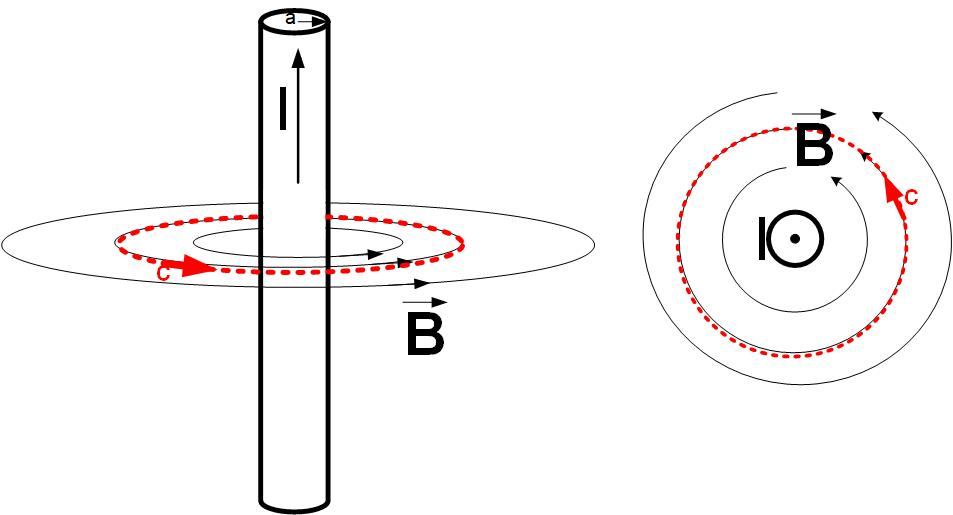
\includegraphics[scale=0.4]{../jpg/AmperesLaw1.jpg}
\end{center}
\caption{ Application of Ampere's law outside an infinite straight conductor}
\label{fig:AmpereOutside}
\end{figure}


We can now apply Ampere's law to a contour inside the wire, as shown in Figure \ref{fig:AmpereInside}. 
We then choose a contour c that is a circle of radius r, but this time, $r<a$. 




\begin{equation}
\oint_c \vec{H} \cdot \vec{dl} = I_{part}
\end{equation}


The current in the above equation is the current enclosed by the contour c. In this case, only the portion of the total current I  is flowing through the contour. 

We can find the current flowing through the contour by using a proportion since the current density is constant through the wire cross-section.

\begin{eqnarray}
\frac{I_{part}}{r^2 \pi}=\frac{I}{a^2 \pi} \\
I_{part}=I \frac{r^2}{a^2}
\end{eqnarray}


Using the same reasoning as in the previous part of the problem, we find that the left side of Ampere's law is $H 2 \pi r$:

\begin{eqnarray}
H 2 \pi r = I \frac{r^2}{a^2} \\
H(r)=I \frac{r}{2 \pi a^2}
\end{eqnarray}

We see that when $r<a$, the magnetic field increases linearly from zero at the axis of the wire to the maximum value of $H(a)=I \frac{1}{2 \pi a}$


\begin{figure}[!ht]
\begin{center}
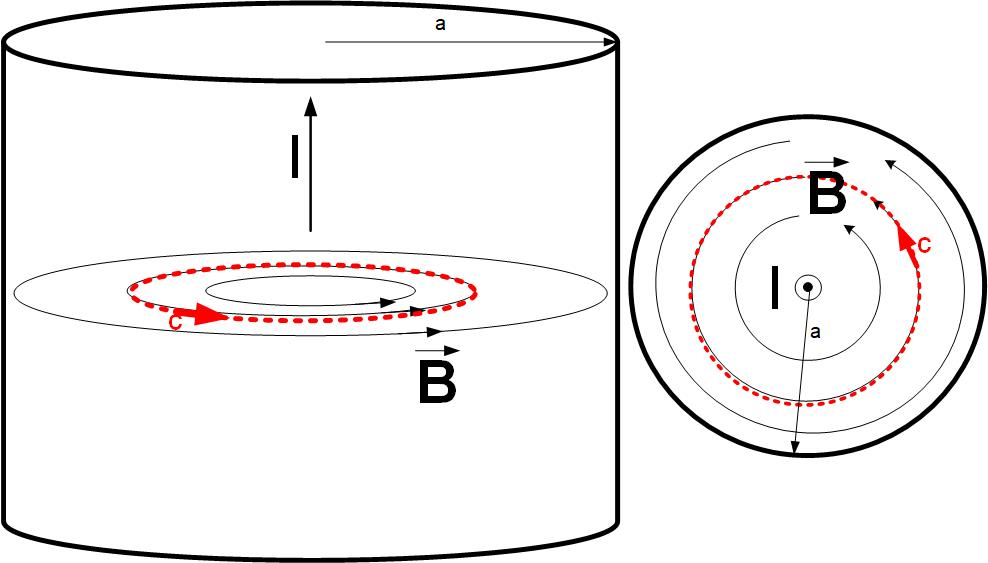
\includegraphics[scale=0.5]{../jpg/AmperesLaw2.jpg}
\end{center}
\caption{Application of Ampere's law inside an infinite straight conductor}
\label{fig:AmpereInside}
\end{figure}



\end{explanation}

\end{example}

\begin{example}
The magnetic field of a solenoid

Find the magnetic field of a solenoid with N turns of uniformly, densely wound wire around an air core, as shown in Figure\ref{fig:solenoid}. The length of the solenoid is L, and the current flowing through the wire is I.  

\begin{explanation}

To find the magnetic field inside the solenoid, we apply Ampere's law to a contour shown in Figure \ref{fig:solenoid}. Using a similar discussion as before, we find that the line integral of the magnetic field along the square loop l is 

\begin{eqnarray}
H l = N' I
\end{eqnarray}

Where N' represents the number of windings enclosed by the contour. Since the solenoid is uniformly wound, 
$N'/l=N/L$, $N'=N l/L$. l is the length of the contour, L is the solenoid's length, and N is the total number of windings.


\begin{eqnarray}
H  l = \frac{N l I}{L} \\
H = \frac{N I}{L} 
\end{eqnarray}

\begin{figure}[ht]
\begin{center}
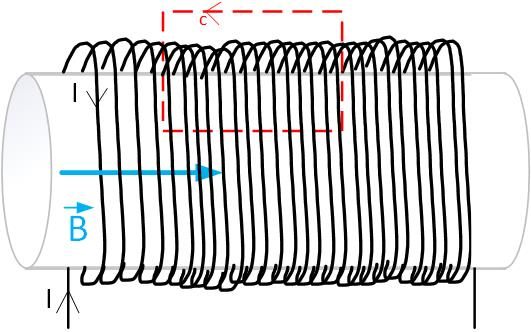
\includegraphics[scale=0.5]{../jpg/Solenoid.jpg}
\end{center}
\caption{Application of Ampere's law to a solenoid.}
\label{fig:solenoid}
\end{figure}


\end{explanation}
\end{example}


\begin{example}
The magnetic field of a toroid

Find the magnetic field inside and outside of a toroid with inner radius a and outer radius b. A toroid is a donut-shaped form, as shown in Figure \ref{fig:toroid}. The wire wound on the toroid carries a current I, and there are N dense, uniform windings on the air core.


\begin{explanation}
 
If we chose a contour outside of the toroid, we see that N windings of current penetrate the contour's surface twice. Once down into the surface, and the other time going up out of the surface. Therefore, the right side of Ampere's law has 2N currents that cancel each other, and the magnetic field is zero.

If we choose a contour inside the toroid's hollow part, there is no current enclosed by the contour. Therefore, the current and the magnetic field are zero.

If we choose a contour inside the toroid, we see that the current penetrates the surface N times. Therefore, Ampere's law states:



\begin{equation}
\oint_c \vec{H} \cdot \vec{dl} = N I
\end{equation}

We again evaluate the left side of the above equation along a circular contour in the magnetic field direction.

\begin{eqnarray}
H 2 \pi r = N I \\
H(r) =\frac{N I}{ 2 \pi r}
\end{eqnarray}



\begin{figure}[htbp]
\begin{center}
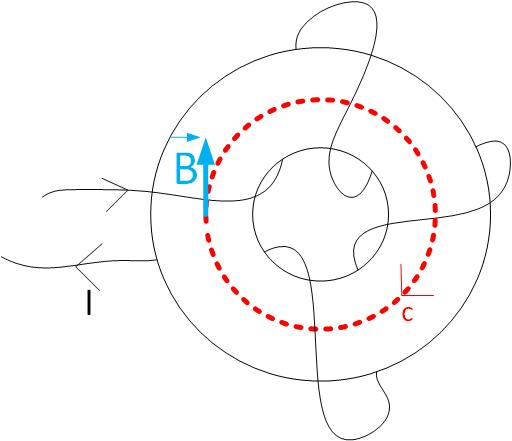
\includegraphics[scale=0.5]{../jpg/toroid.jpg}
\end{center}
\caption{Application of Ampere's law to a toroid.}
\label{fig:toroid}
\end{figure}


\end{explanation}

\end{example}


\end{document} 

